\section {Approach}

We implemented two commenting systems. The first commenting system is MindMargin with anchored comments on a horizontal infinite scroll next to the reference medium (see Figure \ref{fig:frontend}). The second commenting system is a traditional vertical interface (see Figure \ref{fig:traditional}). The two prototypes consist of clean user interfaces to avoid design clutter and distraction. 

MindMargin is split into two sides: The reference media on the left and and an adjacent commenting system on the right. The commenting system displays comments in a horizontal infinite scroll. Thus, an unrestricted amount of comments can be linked to the reference media. Navigation within the infinite scroll component can be performed via mousewheel interaction (either left/right or top/down scrolling with the same effect) or by adjustment of a slider on the bottom of the right split screen. While navigating through the infinite scroll, the reference medium remains fixed on the left. Similar to~\cite{FluidDocs, NB}, comments are anchored to the horizontal reference point of the media. We minimize disturbance by avoiding interactions with the primary text, as defined by~\cite{FluidDocs}, and using thin dotted lines for anchoring to the article's right edge. This design decision was motivated by MindMargin's inherently more visible and thus distracting interface than the traditional vertical system's. 

If a comment has replies, a dropdown button appears on the comment's footer. Lighter in color, replies to comments appear vertically under their comment when the button is clicked. This arrangement optimizes horizontal real estate by reserving horizontal space for parent comments. Readers can upvote and downvote comments. Most recent comments and most popular comments are displayed directly next to the reference media for increased visibility.

\marginpar{
\begin{figure}
  \begin{center}
  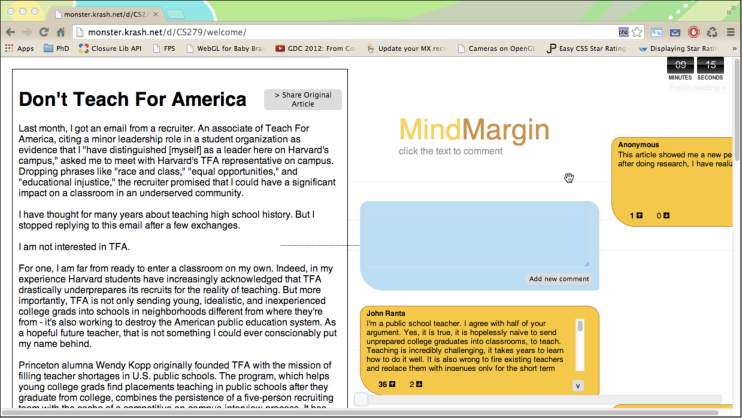
\includegraphics[width=\marginparwidth]{mindmargin.png}
  \caption{The MindMargin system with the reference media on the left and an adjacent commenting system on the right.}
  \label{fig:frontend}
  \end{center}
\end{figure}
}

\marginpar{
\begin{figure}
  \begin{center}
  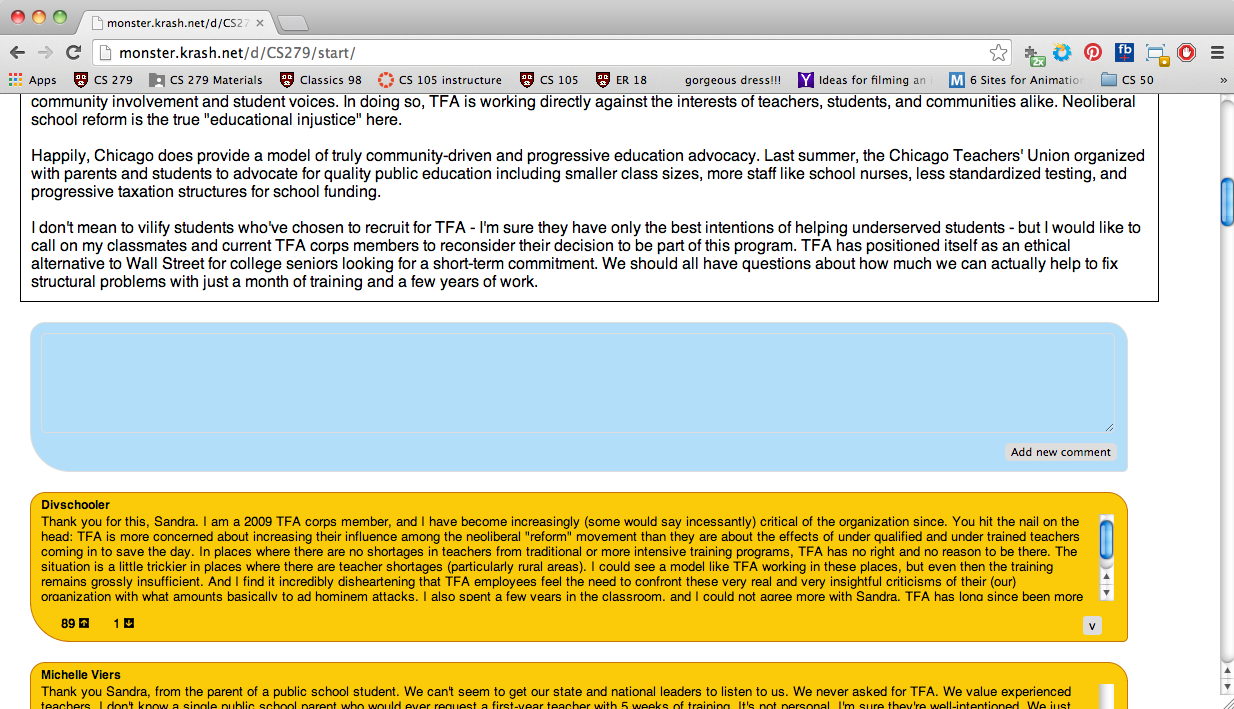
\includegraphics[width=\marginparwidth]{traditional.png}
  \caption{The traditional commenting system with a vertically ordered design.}
  \label{fig:traditional}
  \end{center}
\end{figure}
}
   
Our implementation of the traditional vertical commenting system follows a vertically ordered design: The reference media appears first and on top of the commenting system that follows below. Navigation within the article as well as within the comments can be performed via top/down scrolling. The replies, upvoting, and downvoting function and are organized in the same manner as MindMargin.